\chapter{Introduction}
\renewcommand{\baselinestretch}{\mystretch}
\label{chap:Intro}
%\setlength{\parindent}{0pt}
\PARstart{M}{odern} hardware design and verification are heavily reliant on the hardware synthesis tool (HST), for example, Modelsim, Vivado and Yosys \cite{hardsyntool}. It transforms the HDL file into a netlist based on some criteria, for example, reducing the number of nodes or logical level. Nane et al.'s research conducted a comprehensive analysis of popular HLS tools in both industry and academia, and benchmarks show that they have different degrees of imprecise synthesis \cite{toolsevaulation}. Due to the trade-off between synthesis time and synthesis accuracy, the bug existence possibility of a hardware synthesis tool is high. Actually, many incorrect generations are related to the synthesis tool's vulnerabilities rather than invalid HDL code \cite{torjans}. 

As a consequence, it is crucial to design a test algorithm for HST to guarantee the correctness of synthesis. If there is a bug in the hardware synthesiser, it will produce a wrong synthesis result which may cause substantial financial loss in industry or academic errors in academia. In order to solve the above problem, this project proposes and implements a grey-box fuzz testing to verify hardware synthesis tool.



\section{Motivation}
First of all, the high reliability of HSL is essential in producing correct circuits. Hoang M. et al. have shown that most of the incorrect generations are related to bugs (malicious implanted Trojans or negligent loophole) in the synthesis tool rather than invalid HDL code \cite{torjans}. Despite the development of self-verification, external testing is still necessary. Third-party verification and testing may improve the HST's quality.
%For instance, Intel did not find the floating-point division (FDIV) bug in thour Pentium processor was discovered by Prof. Thomas R. Nicely at Lynchburg College \cite{Intelbug}. Due to this bug, the processor may process a wrong result when dividing a number. The incorrect calculated result occurring probability is 1 in 9 billion FDIV with random parameters. Although the occurring probability is low, it costs Intel company approaching 475 million dollars to recall the defect processors and replace them. 


Secondly, the existing testing tool has several limitations. The coverage of the generated test cases is narrow. For the existing synthesis tool testing software, VlogHammer \cite{wolf2016yosys} concentrates on generating combinatorial circuits with a small number of ports and terminals. It lacks large scale inputs and sequential circuit generation.

Besides, this project has potential value in future development combined with big data analytics. Big data can be applied in predictive analytics and user behaviour analytics, which offers adequate statistical power. In future, fuzzer's bugs detection and identification ability can be enhanced by big data analytics. This cross-subject analysis may guide the development of fuzz testing.

\section{Fuzzing in hardware synthesis}
In conventional hardware design, the truth table and boolean expression need to be simplified manually and realised in real logical gate circuit. This process is cumbersome and error-prone. By working in a high virtual abstract level (only specific the logic functions) and involving computer-aided design (CAD), the design efficiency can be greatly improved and design errors can be reduced \cite{harris2015digital}. In modern industry, HDL such as Verilog, SystemVerilog and VHSIC (Very High Speed Integrated Circuit) Hardware Description Language (VHDL) are used to describe the digital circuits. As a mainstream HDL, Verilog was standardised as IEEE 1364 in 2009 \cite{1620780} which occupied a large market share in the industry and commercial application area. In 2009, Verilog standard (IEEE 1364-2005) was merged with SystemVerilog standard and officially became a part of SystemVerilog. Since then, a new standard was formed (IEEE 1364-2005). Comparing with VHDL, Verilog has more compact statements and more flexibility. As a consequence, Verilog was selected as the HDL in this project. The HDL code file needs to be transformed into a netlist by a HST, for example, VIVADO and ModelSim.\label{ieeestandard}

Fuzz testing, also known as fuzzing, is a kind of software test technique that involves providing invalid, unexpected or random data to a compiler \cite{miller2007fuzz}. For its quality assurance aspect, fuzz testing is efficient in finding coding errors and security loopholes in the compiler or higher-level components (operating systems and networks). With a large amount of random input data, the DUT might attempt to crash or suffering memory overflow issue. If a bug is detected, the potential cause of this will be also needed to be identified. This includes locate the source file of bug and match the bug's character with the reference table. The ''fuzzer'' is defined to generate a large number of random inputs and identify the potential cause of bugs. According to acknowledge of DUT's inside structure, the fuzzer can be categorised as white-box, grey-box or black-box.

In 1989, fuzz testing algorithm was initially proposed by Barton Miller at University of Wisconsin \cite{miller2007fuzz}. He designed a fuzzer to automatically generate random file and command lines in testing utilities of Unix-based software. He also designed a debugging tool to identify the cause of crash. As presented in his paper \cite{miller1990empirical}, 25-33\% of the utility programs on a different version of UNIX system were crashed during the fuzz testing. Above results show that this testing algorithm is useful to find the bugs that existed in the DUT. At present, the definition of term fuzz testing is not limited in teasing command-line utilities.

Although, fuzz testing algorithm has weakness in not robust targeted bug-finding. 
With simple design structure, high practicability and capability, it has an impressive cost-efficient ratio in debugging area to discover severe overlooked defects. Different from other testing algorithm and method, it has an advantage in no need oracle for test results. For software testing, the main application of this testing algorithm is to discover vulnerabilities such as buffer overflow,
denial of service (DOS), cross-site scripting and structured query language (SQL) injection\cite{Yang:2011:FUB:1993316.1993532}. 

Based on the above discussions, the purpose of this project is to apply this fuzz testing algorithm in HST. With the trend of open source project (OPS), this project is focusing on low-level open-source hardware synthesis software, for example, ABC and SIS. The randomly generated HDL files will be entered to a hardware synthesis software by a Linux shell program. Inspired by Xuejun Yang and his colleagues designed Csmith \cite{Yang:2011:FUB:1993316.1993532}, the basic block diagram of this project has been shown in Fig \ref{Fig:Block diagram}. GNC compiler collection (GCC) and Microsoft's Visual studio (MSV) are C compilers in the upper figure. For the bottom figure, ABC and SIS are hardware synthesis software. Different from the software fuzz testing, the input netlist file can be directly compared with the output of HST because these two files have same format. I Comparing the synthesised netlist with its original input circuit, if these two circuits are not equivalent, it indicates that there might be a bug in the tested tool. 


\begin{figure}[htb]
\centering
\begin{minipage}[htb]{1\textwidth}
\centering
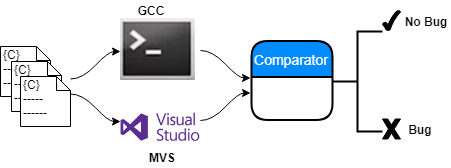
\includegraphics[width=8.5cm]{MScThesisTemplate/Figs/1.pdf}
\end{minipage}
\begin{minipage}[htb]{1\textwidth}
\centering
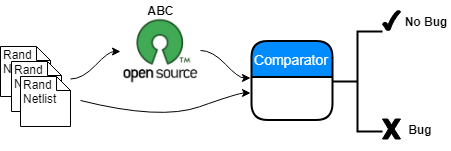
\includegraphics[width=8.5cm]{MScThesisTemplate/Figs/2.pdf}
\end{minipage}
\caption{\footnotesize Block diagram}
\label{Fig:Block diagram}
\end{figure}

\section{Project Contribution}
The main contributions of this project are:
\begin{itemize}
    \item Applying the fuzz testing algorithm in open-source HST testing field. The fuzz testing method was advanced and extended. The randomly generated file has better coverage and more esoteric comparing to typical Verilog code file generated by the existing testing tool.
    \item Detected bugs and crash issues were analysed through qualitative and quantitative methods. Bug analysis not only benefits the debug and version upgrade of the HST, but also worthy in big data research in bug-hunting. 
    \item With further polishing, the designed testing tool can be promoted as a distributed Linux software in a collaborative public manner.
\end{itemize}

\section{Thesis Outline}
This thesis is divided into six chapters to illustrate the design and implementation of fuzzing netlist. Following the first introduction, background Chapter 2 will demonstrate the theory applied in this project and related work. Chapter 3 discusses project planning, including the objectives, methodology and the strategy for evaluating the project. In Chapter 4, the detail implementation of the combinational and sequential testing circuit are described. The shell script program with error detection will also be presented. The results of the designed fuzzer and tool-flow will be depicted and evaluated in Chapter 5. In the final chapter, it concludes the impact of the project and future work. 
